\chapter{Utilização do Vortex} 
\label{Utilização}

A criação de um novo projeto com o \textit{framework} Vortex pode ocorrer por meio de duas abordagens: a clonagem do projeto base no repositório oficial do Vortex no Github \footnote{https://github.com/mex3890/vortex.git} ou a execução do comando apresentado na seção \ref{packagist_command}. Após a clonagem do projeto, é suficiente executar o comando de instalação do Composer:

\spaceH{}
\lstinputlisting[language=bash,caption=Clonagem do repositório Vortex e instalação de dependências]{scripts/clone_vortex_project.bash}
\label{scripts/clone_vortex_project.bash}

\section{Criação do Projeto}\label{packagist_command}

Para criar um novo projeto através do Composer, é necessário dispor de um ambiente PHP compatível com a versão específica utilizada do framework, ou, caso não seja especificada, será utilizada a versão mais recente. Além disso, é indispensável fornecer um nome para o projeto a ser criado. O comando correspondente está disponível em Vortex Packagist \footnote{https://packagist.org/packages/vortex-framework/vortex}.

\spaceH{}
\lstinputlisting[language=bash,caption=Criação projeto Vortex com comando Packagist]{scripts/create_project_from_packagist.bash}
\label{scripts/create_project_from_packagist.bash}

\section{Configuração do Ambiente}

Com o projeto baixado será necessário a criação do arquivo de configuração de ambiente (.env), o projeto possui um arquivo de exemplo (\ref{scripts/app_environment_example.env}) que deve ser usado como base, este arquivo fica na raiz do projeto. As variáveis devem ser preenchidas com os valores referentes ao ambiente em que está, o arquivo tem o padrão abaixo.

\spaceH{}
\lstinputlisting[language=bash,caption=Exemplo de arquivo de configuração de ambiente]{scripts/app_environment_example.env}
\label{scripts/app_environment_example.env}

\section{Instalação das Dependências}

Ao criar um novo projeto via Composer, as dependências do PHP já são instaladas, porém as dependências do NPM não, logo o comando abaixo instala todas as dependências do PHP, NPM e cria as tabelas necessárias na base de dados configurada no arquivo de configuração de ambiente(.env).

\spaceH{}
\lstinputlisting[language=TeX,caption=Comando de instalação de dependências]{scripts/vortex_installation_command.bash}
\label{scripts/vortex_installation_command.bash}

Observe que ao final do comando, caso alguma etapa falhe, esta etapa é mostrada em vermelho. Em caso de falha nas “migrations” deve-se verificar as configurações relativas ao banco de dados no arquivo de configuração de ambiente (.env) ou verificar se as tabelas geradas pela instalação já não foram criadas.

\section{Teste do Ambiente}

Para verificar se a instalação e a configuração ocorreu do jeito esperado o comando abaixo serve para testar a aplicação em um servidor local embutido do PHP:

\spaceH{}
\lstinputlisting[language=TeX,caption=Comando para iniciar servidor embutido PHP]{scripts/vortex_server_start_command.bash}
\label{scripts/vortex_server_start_command.bash}

Ao acessar o domínio na porta definida no arquivo de configuração de ambiente verifica-se a página inicial do \textit{framework}.

\begin{figure}[ht]
\centering
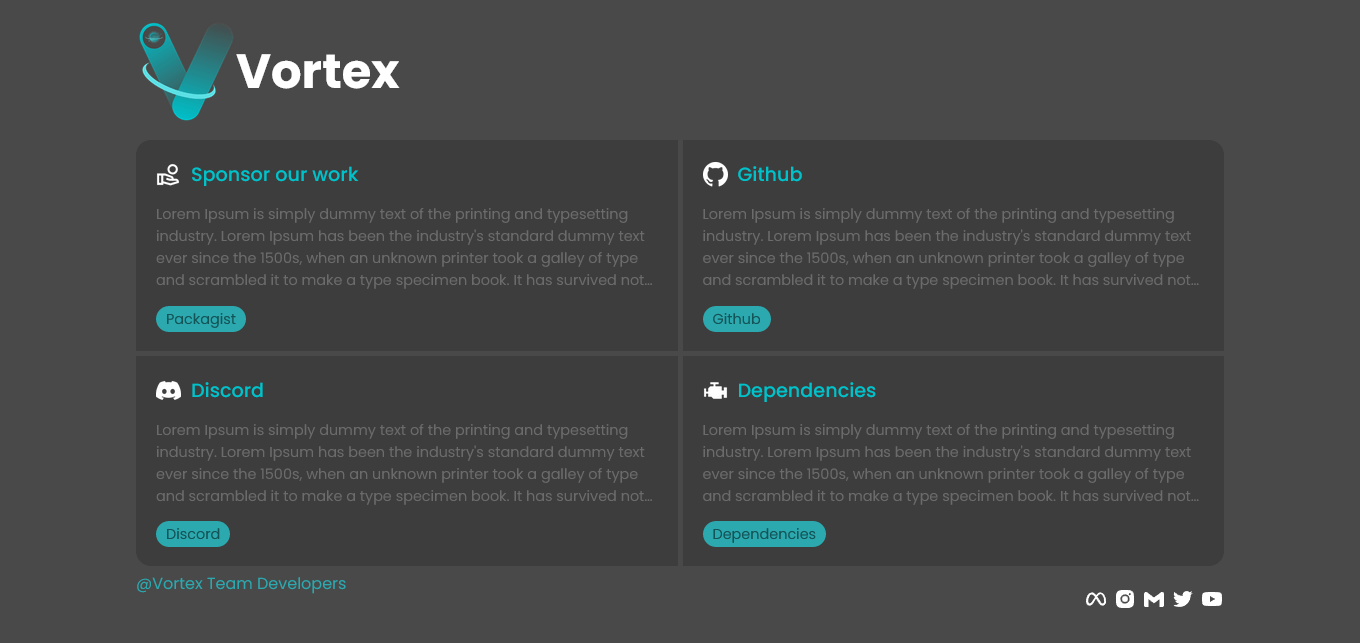
\includegraphics[width=15cm]{figures/first_page_vortex_screenshot.png}
\caption{Página inicial de um projeto com Vortex Framework}
\label{first_page_vortex_screenshot.png}
\end{figure}

\section{Interface de Linha de Comando}
\paragraph{}
O Vortex possui comandos administrados pelo gerênciador de comandos, Cosmo. Os comandos foram agrupados por afinidade, para acessar o Cosmo basta utilizar o seguinte comando no terminal na raiz do projeto:

\spaceH{}
\lstinputlisting[language=bash,caption=Comando para listagem de comandos do Cosmo]{scripts/cosmo_commands_list.bash}
\label{scripts/cosmo_commands_list.bash}

Para utilizar os comandos disponíveis no Cosmo, basta usar o comando anterior mais o comando específico. Todo comando possui a opção ''--\textit{help}'', que retorna uma breve descrição do comando juntamente com seus parâmetros.

\spaceH{}
\lstinputlisting[language=bash,caption=Comando para busca de ajuda de um comando específico]{scripts/cosmo_help_commands.bash}
\label{scripts/cosmo_help_commands.bash}

\section{Comandos Vortex}
Vortex disponibiliza um grupo de comandos que ajudam na configuração e execução do ambiente da aplicação, nenhum destes comandos é obrigatório para o funcionamento da aplicação, porém eles facilitam e realizam o que o projeto precisa para funcionar como foi idealizado.

\subsubsection{vortex:install}
O comando abaixo instala todas as dependências necessárias para começar a aplicação, caso a aplicação tenha sido criada a partir do comando \ref{scripts/clone_vortex_project.bash} as dependências administradas pelo Composer já estão instaladas porém os pacotes do NPM e as tabelas necessárias para o funcionaemnto do \textit{framework} não estão instaladas.

\spaceH{}
\lstinputlisting[language=bash,caption=Comando para instalação de dependências]{scripts/cosmo_vortex_install.bash}
\label{scripts/cosmo_vortex_install.bash}

\subsection{vortex:server}

Este comando utiliza a porta configurada no arquivo de ambiente (.env) para executar o servidor embutido do PHP no projeto.

\spaceH{}
\lstinputlisting[language=bash,caption=Comando para iniciar servidor embutido PHP]{scripts/cosmo_vortex_server.bash}
\label{scripts/cosmo_vortex_server.bash}

\subsection{Geração de chave única}

Para gerar a chave única do projeto que é usada em encriptações e validações de requisições, utilize o comando abaixo. Esta chave será gerada e armazenada no arquivo de configuração de ambiente (.env), na raiz do projeto.

\spaceH{}
\lstinputlisting[language=bash,caption=Comando para gerar chave única da aplicação]{scripts/cosmo_key_generate.bash}
\label{scripts/cosmo_key_generate.bash}

\section{Publicação de recursos}

Para publicar recursos internos ou opcionais, utilize o comando abaixo, ao usar o comando, uma lista de opções será mostrada, ao escolher uma opção, o recurso será publicado.

\spaceH{}
\lstinputlisting[language=bash,caption=Comando para publicação de recursos]{scripts/cosmo_publish.bash}
\label{scripts/cosmo_publish.bash}

\begin{figure}[ht]
\centering
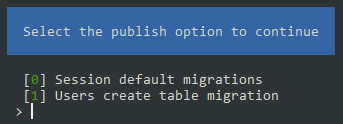
\includegraphics[width=15cm]{figures/publish_command.png}
\caption{Lista de opções ao utilizar o comando de publicação de recursos}
\label{Fig02}
\end{figure}

\subsection{Comandos de Criação}

Os comandos de criação funcionam basicamente da mesma forma, gerando arquivos específicos em diretórios específicos com algumas vantagens em relação a criar classes manualmente, pois adicionam e preenchem atributos e configurações necessárias.

\begin{enumerate}
    \item{Criação de Comandos (\textit{Commands})}
    Cosmo possibilita a criação de rotinas de comandos customizaveis e reutilizaveis através das classes de comandos, para criar uma classe base para um determinado comando utiliza-se o comando abaixo:  

    \spaceH{}
    \lstinputlisting[language=bash,caption=Comando para criação de outros comandos]{scripts/cosmo_make_command.bash}
    \label{scripts/cosmo_make_command.bash}

    \item{Criação de Controladoras (\textit{Controller})}
    \paragraph{}
    O comando de criação de controladoras possui a opção ''--api'' ou ''-a'', ao usar esta opção a controladora adicionará apenas os métodos necessários para uma API.

    \spaceH{}
    \lstinputlisting[language=bash,caption=Comando para criação de \textit{controllers}]{scripts/cosmo_make_controller.bash}
    \label{scripts/cosmo_make_controller.bash}

    \item{Criação de Exceções (\textit{Exceptions})}
    O Vortex possui uma classe de adaptação das exceções nativas do PHP que permitem a opção de adicionar a ocorrencia desta exceção no log da aplicação ou não.
    
    \spaceH{}
    \lstinputlisting[language=bash,caption=Comando para criação de \textit{exceptions}]{scripts/cosmo_make_exception.bash}
    \label{scripts/cosmo_make_exception.bash}

    \item{Criação de Fábricas (\textit{Factories})}
    As classes fábricas tem a finalidade de definir a estrutura para a inserção em massa.

    \spaceH{}
    \lstinputlisting[language=bash,caption=Comando para criação de \textit{factories}]{scripts/cosmo_make_factory.bash}
    \label{scripts/cosmo_make_factory.bash}

    \item{Criação de Observadores (\textit{Observers})}

    \spaceH{}
    \lstinputlisting[language=bash,caption=Comando para criação de \textit{observers}]{scripts/cosmo_make_observer.bash}
    \label{scripts/cosmo_make_observer.bash}

    \item{Criação de \textit{Middlewares}}

    \spaceH{}
    \lstinputlisting[language=bash,caption=Comando para criação de \textit{middlewares}]{scripts/cosmo_make_middleware.bash}
    \label{scripts/cosmo_make_middleware.bash}

    \item{Criação de Migrações (\textit{Migrations})}

    \spaceH{}
    \lstinputlisting[language=bash,caption=Comando para criação de \textit{migrations}]{scripts/cosmo_make_migration.bash}
    \label{scripts/cosmo_make_migration.bash}

    \item{Criação de Modelos (\textit{Models})}

    \spaceH{}
    \lstinputlisting[language=bash,caption=Comando para criação de \textit{models}]{scripts/cosmo_make_model.bash}
    \label{scripts/cosmo_make_model.bash}

    \item{Criação de Sementes (\textit{Seeds})}

    \spaceH{}
    \lstinputlisting[language=bash,caption=Comando para criação de \textit{seeds}]{scripts/cosmo_make_seed.bash}
    \label{scripts/cosmo_make_seed.bash}

    \item{Criação de Serviços (\textit{Services})}

    \spaceH{}
    \lstinputlisting[language=bash,caption=Comando para criação de \textit{services}]{scripts/cosmo_make_service.bash}
    \label{scripts/cosmo_make_service.bash}
\end{enumerate}

\subsection{Comandos de Migrações}

Os comandos desta seção são referentes as migrações do banco de dados como citado em \ref{rt_migrations}. Com eles é possível criar, alterar e excluir tabelas, além de programar alterações pontuais na base de dados, como: alterar o formato de uma coluna de data que armazenava com o formato Y/m/d para Y/m/d H:i:s.

\subsubsection{Execução das Migrações}

Este comando possui a opção de receber o nome das migrações que devem ser executadas, caso nenhuma seja fornecida todas as migrações que ainda não foram executadas serão. Observe que em hipótese nenhuma uma migração é executada mais de uma vez, apenas com o comando de desfazer as migrações será possível executa-las novamente. Os nomes das migrações devem ser passados separados por espaço, como no comando abaixo:

\spaceH{}
\lstinputlisting[language=bash,caption=Comandos para executar \textit{migrations}]{scripts/migration_execution.bash}
\label{scripts/migration_execution.bash}

\subsubsection{Listagem das Migrações}

Comando responsável por verificar todas as \textit{migrations} presentes na aplicação e retornar além da listagem das mesmas o estado atual de cada uma, sendo possível: \textit{already ran} e \textit{needed ran}. A figura \ref{print_migration_list} demonstra um exemplo de \textit{output} deste comando, onde a primeira coluna representa o arquivo desta \textit{migration} e a segunda o estado atual da mesma:

\spaceH{}
\lstinputlisting[language=bash,caption=Comandos para listar \textit{migrations}]{scripts/cosmo_migration_list.bash}
\label{scripts/cosmo_migration_list.bash}

\begin{figure}[H]
\centering
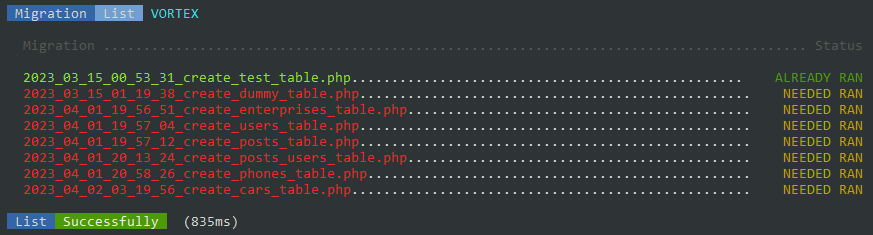
\includegraphics[width=15cm]{figures/print_migration_list.png}
\caption{Exemplo de retorno ao executar comando de listagem de migrações}
\label{print_migration_list}
\end{figure}

\subsubsection{Desfazer Migrações}

Para desfazer o que uma migração executou, utilize o comando abaixo, este comando possui as opções de receber \textit{filename}= nome da migração e step= step para ser desfeito, sempre que o comando de execução das migrações executar um bloco de migrações este bloco receberá o mesmo \textit{step}, e quando desfeito passando o \textit{step} o bloco inteiro será desfeito. Caso nenhum parâmetro for passado, as migrações do último \textit{step} serão desfeitas.

\spaceH{}
\lstinputlisting[language=bash,caption=Comandos para desfazer uma \textit{migration}]{scripts/cosmo_migration_rollback.bash}
\label{scripts/cosmo_migration_rollback.bash}

\subsection{Execução de Sementes}

Para executar as classes semente, que são responsáveis por popular a base de dados, o comando \ref{scripts/cosmo_execute_seed.bash} demonstra esta funcionalidade. Este comando permite a passagem de múltiplas classes sementes, e mandatoriamente necessita de ao menos uma classe semente.

\spaceH{}
\lstinputlisting[language=bash,caption=Comandos para executar \textit{seeds}]{scripts/cosmo_execute_seed.bash}
\label{scripts/cosmo_execute_seed.bash}

\subsection{Listagem de Rotas}

Este comando permite uma visualização organizada de todas as rotas definidas no projeto.

\spaceH{}
\lstinputlisting[language=bash,caption=Comandos para listagem de \textit{routes}]{scripts/cosmo_route_list.bash}
\label{scripts/cosmo_route_list.bash}

\begin{figure}[ht]
    \centering
    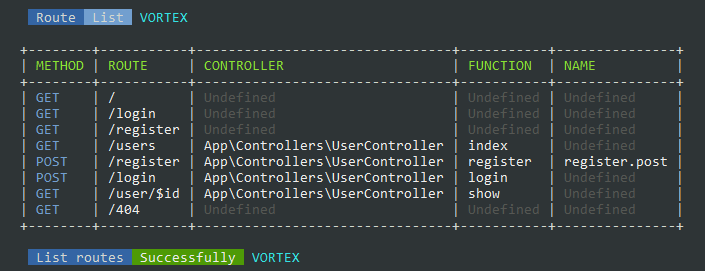
\includegraphics[width=15cm]{figures/print_route_list.png}
    \caption{Exemplo de retorno ao executar comando de listagem de rotas}
\label{print_route_list}
\end{figure}

\subsection{Base de Dados}

Vortex provê alguns comandos para aumentar a produtividade e facilidade na hora da abstração de suas entidades e seus relacionamentos, os comandos a seguir focam principalmente nestes quesitos.

\subsubsection{Visualizador de tabelas}

Este comando serve para uma visualização simples da base de dados, mais especificamente das colunas das tabelas do \textit{schema} cadastrado na aplicação no arquivo de configurações de ambiente.

\spaceH{}
\lstinputlisting[language=bash,caption=Comandos para listagem de tabelas da base de dados]{scripts/cosmo_db_display.bash}
\label{scripts/cosmo_db_display.bash}

\subsubsection{Lista de relacionamentos}

Este comando tem o papel de prover uma pré-visualização dos relacionamentos antes de realizar a "tradução" da base de dados para os relacionamentos disponíveis no Vortex. 

\spaceH{}
\lstinputlisting[language=bash,caption=Comandos para listagem de relacionamentos da base de dados]{scripts/cosmo_db_relationships.bash}
\label{scripts/cosmo_db_relationships.bash}

\subsubsection{Mapeador de Modelos e Relacionamentos}
\label{translate_relations}

O comando de abaixo possui este nome pois realiza a tradução da estrutura da base de dados para a estrutura do \textit{framework}, incluindo seus relacionamentos com os demais modelos. Atualemnte mapeia relacionamentos até o terceiro nível que seria um nível acima de relacionamentos diretos.

\spaceH{}
\lstinputlisting[language=bash,caption=Comandos para tradução das tabelas da base de dados em \textit{models} e seus relacionamentos]{scripts/cosmo_db_translate.bash}
\label{scripts/cosmo_db_translate.bash}

\subsubsection{Engenharia Reversa}

Em casos de migração de projetos feitos em tecnologias diferentes, esse comando permite a geração das migrações automaticamente, baseadas na base de dados. Ainda não estão disponíveis a criação de índices por este comando.

\spaceH{}
\lstinputlisting[language=bash,caption=Comandos para engenharia reversa das tabelas da base de dados em \textit{migrations}]{scripts/cosmo_db_reverse.bash}
\label{scripts/cosmo_db_reverse.bash}

\section{Montador de Consultas (\textit{Query Builder})}
\label{QueryBuilder}

Vortex disponibilza de um montador de consultas roubusto que permite completa abstração da base de dados, juntamente com métodos e classes que facilitam sua utilização.

\subsection{\textit{Select Builder}}

Para descrever a utilização do construtor será usado como base uma tabela de usuários e seus demais relacionamentos que serão descritos em subseções desta seção. Uma consulta simples retornando todos os registros da tabela, neste exemplo usuários, seria feita da forma abaixo, observando que o retorno da consulta será uma \textit{Collection}:

\begin{figure}[ht]
    \centering
    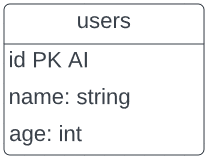
\includegraphics[width=4cm]{figures/users_table.png}
    \caption{Representação tabela de usuários}
\label{users_table}
\end{figure}

\spaceH{}
\lstinputlisting[language=bash,caption=\textit{Query} para realizar uma consulta simples]{scripts/simple_select_query.php}
\label{scripts/simple_select_query.php}

\subsection{Condicionais}

Para utilizar condicionais deve-se sempre partir de um comando principal que inicie uma operação na base de dados, que pode ser: \textit{select(), update() ou delete()}, e sempre serão executadas a partir do método \textit{get()}. Condicionais podem ser encadeadas livremente e infinitamente. 

\subsubsection{\textit{Where}}
\label{where}
\paragraph{}
Para realizar uma condição simples é usado o método ''\textit{where()}''.

\begin{lstlisting}
[..]->where($column,$value,$operator,$table): static
\end{lstlisting}

\begin{table}[ht]
\centering
\vspace{0.5cm}
\begin{tabular}{|c|c|c|c|}
\hline  
Parâmetro & Tipo & ValorPadrão & Descrição \\
\hline 
column   & string     & -    & Coluna a ser comparada    \\
value    & string|int & -    & Valor a ser comparado     \\
operator & string     & '='  & Operador da comparação    \\
table & string|null|bool   & null & Tabela referente a coluna \\
\hline
\end{tabular}
\caption{Parâmetros do método \textit{where()}}
\end{table}

Observe que caso a tabela não seja especificada será utilizada a passada no \textit{select()}. O método pode ser encadeado ilimitadamente, automaticamente se a consulta possuir mais de um \textit{where} ela se resolverá convertendo o mesmo para \textit{and}.

\spaceH{}
\lstinputlisting[language=bash,caption=\textit{Query} para realizar uma consulta com múltiplas condições]{scripts/query_multiple_conditions.php}
\label{scripts/query_multiple_conditions.php}

A sintaxe para utilizar o método com o operador \textit{like} é como o exemplo abaixo, é necessário colocar explicitamente os marcadores de porcentagem no valor que será comparado.

\spaceH{}
\lstinputlisting[language=bash,caption=\textit{Query} para realizar uma consulta com operador \textit{like}]{scripts/query_with_like_condition.php}
\label{scripts/query_with_like_condition.php}

\subsubsection{\textit{orWhere}}

O método \textit{orWhere()} segue o mesmo modelo do método anterior, \ref{where} e com os mesmos parâmetros porém como o próprio nome do método descreve ele realizara uma comparação com \textit{OR}. Note que em SQL não faz sentido uma comparação \textit{OR WHERE} sem outra comparação anterior, porém caso o método seja chamado sozinho a consulta será automaticamente alterada para um \textit{where} simples, evitando possiveis erros de sintaxe.

\spaceH{}
\lstinputlisting[language=bash,caption=\textit{Query} para realizar uma consulta com operador \textit{or}]{scripts/query_with_or_where.php}
\label{scripts/query_with_or_where.php}

\subsubsection{\textit{whereNot}}

Possui a mesma estrutura do método \textit{where()} porém a expressão final que será montada terá estrutura no formato ''\textit{WHERE ID NOT = 10}''.

\spaceH{}
\lstinputlisting[language=bash,caption=\textit{Query} para realizar uma consulta com \textit{where not}]{scripts/query_where_not.php}
\label{scripts/query_where_not.php}

\subsubsection{\textit{whereBetween}}
\label{whereBetween}

Este método deve ser usado para realizar uma consulta em um intervalo explicito, note que assim como os demais métodos citados anteriormente o parâmetro ''\textit{table}'' também está presente.

\spaceH{}
\lstinputlisting[language=bash,caption=\textit{Query} para realizar uma consulta com \textit{where between}]{scripts/query_with_where_between.php}
\label{scripts/query_with_where_between.php}

\subsubsection{\textit{whereNotBetween}}

Assim como o método anterior \ref{whereBetween}, o ''\textit{whereNotBetween}'' realiza uma consulta em um intervalo, porém neste caso retornará o que não estiver neste intervalo, assim como sua utilização referente na linguagem SQL.

\spaceH{}
\lstinputlisting[language=bash,caption=\textit{Query} para realizar uma consulta com \textit{where not between}]{scripts/query_with_where_not_between.php}
\label{scripts/query_with_where_not_between.php}

\subsubsection{\textit{whereIsNull}}
\label{whereIsNull}

Este método recebe uma coluna como parâmetro e utiliza esta coluna para consultar se o valor dela igual a nulo, e retornará apenas os registros que tiverem esta coluna nula.

\spaceH{}
\lstinputlisting[language=bash,caption=\textit{Query} para realizar uma consulta com \textit{where is null}]{scripts/query_with_where_is_null.php}
\label{scripts/query_with_where_is_null.php}

\subsubsection{\textit{whereIsNotNull}}

Funcionamento igual o método \ref{whereIsNull} descrito anteriormente, mas fazendo o inverso, retornando apenas os registros que não possuirem a coluna nula.


\lstinputlisting[language=bash,caption=\textit{Query} para realizar uma consulta com \textit{where is not null}]{scripts/query_with_where_is_not_null.php}
\label{scripts/query_with_where_is_not_null.php}

\subsubsection{\textit{whereAll}}

Para realizar uma consulta onde somente serão retornados os registros caso todos os resultados de uma subconsulta respeitem uma determinada condição usa-se o ''\textit{whereAll}''. 

\lstinputlisting[language=bash,caption=\textit{Query} para realizar uma consulta com \textit{where all}]{scripts/query_with_where_all.php}
\label{scripts/query_with_where_all.php}

\subsubsection{\textit{whereAny}}

Quando a consulta deve retornar somente caso pelo menos um registro de uma subconsulta respeite uma determinada condição deve-se usar o ''\textit{whereAny}'' como no exemplo abaixo:

\spaceH{}
\lstinputlisting[language=bash,caption=\textit{Query} para realizar uma consulta com \textit{where any}]{scripts/query_with_where_any.php}
\label{scripts/query_with_where_any.php}

\subsubsection{\textit{whereIn}}

Para realizar uma consulta que deve retornar registros apenas quando estiverem dentro do retorno de outra subconsulta ou em um vetor de valores.

\spaceH{}
\lstinputlisting[language=bash,caption=\textit{Query} para realizar uma consulta com \textit{where in}]{scripts/query_with_where_in.php}
\label{scripts/query_with_where_in.php}

\subsubsection{\textit{whereNotIn}}

Para retornar os valores que não estão em um subconsulta ou em um vetor devemos utilizar o método ''\textit{whereNotIn}'' com uma função anônima ou um vetor de valores da coluna especificada.

\spaceH{}
\lstinputlisting[language=bash,caption=\textit{Query} para realizar uma consulta com \textit{where not in}]{scripts/query_with_where_not_in.php}
\label{scripts/query_with_where_not_in.php}

\subsubsection{\textit{whereExists}}

Este método irá retornar apenas os registros que tiverem algum retorno na subconsulta, ou seja apenas os registros com algum valor associado na subconsulta será retornado.

\spaceH{}
\lstinputlisting[language=bash,caption=\textit{Query} para realizar uma consulta com \textit{where exist}]{scripts/query_with_where_exist.php}
\label{scripts/query_with_where_exist.php}

\subsubsection{\textit{when}}

Quando precisamos condicionar a realização de uma condicional a uma variável ou proposição booleana utilizaremos o ''\textit{when}''.

\spaceH{}
\lstinputlisting[language=bash,caption=\textit{Query} para realizar uma consulta com \textit{when}]{scripts/query_with_when.php}
\label{scripts/query_with_when.php}

\subsection{Relacionamento entre tabelas (\textit{table joins})}
Para realizar a conexão entre duas tabelas usamos os SQL ''\textit{joins}''. Os métodos que realizam estas operações possuem basicamente a mesma estrutura e parâmetros, com algumas ressalvas que serão abordadas a seguir. A tabela \ref{tab:joins}  contem os métodos destas operações.

\begin{table}[ht]
\centering
\vspace{0.5cm}
\begin{tabular}{|c|c|c|c|}
\hline  
Método & Join & Parâmetros \\
\hline 
innerJoin   & INNER JOIN & string table, closure callback \\
leftJoin    & LEFT JOIN  & string table, closure callback \\
rightJoin   & RIGHT JOIN & string table, closure callback \\
fullJoin    & FULL JOIN  & string table, closure callback \\
crossJoin   & CROSS JOIN & string table                   \\
\hline
\end{tabular}
\caption{Métodos para relacionar tabelas}
\label{tab:joins}
\end{table}

\lstinputlisting[language=bash,caption=\textit{Query} para realizar uma consulta com \textit{inner join}]{scripts/query_with_join.php}
\label{scripts/query_with_join.php}

O método \textit{''crossJoin()''} permite apenas passar o nome da tabela que será unida, tendo em vista que o SQL \textit{''CROSS JOIN''} realiza um produto cartesiano entre as duas tabelas.

\subsection{Filtros de consultas}

\subsubsection{Ordenar por colunas (\textit{''Order By''})}

Para ordenar consultas por uma determinada coluna, utilize o método \textit{''orderBy()''}. Est método de ordenação pode ser utilizado de formas diferentes, a primeira é quando deve-se ordenar apenas por uma coluna de forma crescente.

\spaceH{}
\lstinputlisting[language=bash,caption=\textit{Query} para realizar uma consulta com \textit{order by}]{scripts/query_with_order_by.php}
\label{scripts/query_with_order_by.php}

Para explicitar qual a direção que deve ocorrer a ordenação, utiliza-se um vetor associativo onde a chave é a coluna da tabela e o valor deve indicar a direção, sendo as seguintes opções possíveis: \textit{''DESC''} (decrescente), \textit{''ASC''} (ascendente) e \textit{''null''} (nulo). Este último se da quando não há necessidade de explicitar a direção, logo o SGBD determinará a direção padrão, no MySQL, por exemplo, é ascendente.

\spaceH{}
\lstinputlisting[language=bash,caption=\textit{Query} para realizar uma consulta com \textit{order by} e suas variações]{scripts/query_with_order_by_variations.php}
\label{scripts/query_with_order_by_variations.php}

\subsubsection{Agrupar por colunas (\textit{group by})}

Utiliza-se o método \textit{''groupBy()''} quando há a necessidade de agrupar registros pelo valor de uma determinada coluna ou colunas, este método pode receber por parâmetro o nome de uma coluna ou um vetor de colunas.

\spaceH{}
\lstinputlisting[language=bash,caption=\textit{Query} para realizar uma consulta com \textit{group by}]{scripts/query_with_group_by.php}
\label{scripts/query_with_group_by.php}

\subsubsection{Limitador de registros (\textit{limit})}

Limita o número de registros que serão retornados, quando passado por parâmetro apenas o primeiro parâmetro (\textit{''$count$''}) este será o número de registros a serem retornados, contando a partir do primeiro registro. Já quando o segundo é passado teremos o valor por onde essa contagem de registros será iniciada, como nos exemplos abaixo:

\spaceH{}
\lstinputlisting[language=bash,caption=\textit{Query} para realizar uma consulta com \textit{limit}]{scripts/query_with_limit.php}
\label{scripts/query_with_limit.php}

No primeiro exemplo seriam retornados os cinco primeiros registros, contando a partir do primeiro. No segundo teremos também cinco registros porém sendo contados a partir do segundo registro, funcionalidade muito utilizada em paginações.

\subsubsection{Condicionando agregações (\textit{Having})}

Para utilizar a expressão SQL \textit{''HAVING''} o Vortex possue o método com a sintaxe mostrada no código \ref{scripts/query_with_having.php}. Este método permite múltiplas condições que são passadas em sua função anônima que deve ser passada por parâmetro e possue mandatoriamente um parâmetro que deve ser uma instância da classe HavingBuilder. Os métodos disponíveis para novas condições dentro da instância do HavingBuilder são \textit{''and()''} e \textit{''or()''}

\spaceH{}
\lstinputlisting[language=bash,caption=\textit{Query} para realizar uma consulta com \textit{having}]{scripts/query_with_having.php}
\label{scripts/query_with_having.php}

\subsubsection{\textit{First}}

O método \textit{''first()''} garante que a consulta retornará o primeiro elemento consultado, caso ele exista, este método deve ser encorajado por realizar um \textit{''LIMIT (1)''} que melhora a performance quando precisa-se apenas do primeiro elemento.

\spaceH{}
\lstinputlisting[language=bash,caption=\textit{Query} para realizar uma consulta com \textit{first}]{scripts/query_with_first.php}
\label{scripts/query_with_first.php}

\subsubsection{\textit{Last}}
Para retornar o último registro da consulta utilize o método \textit{''last()''}, este método aceita como parâmetro que representa a coluna que será usada para ordenar os registros, caso esta coluna não seja passada, o último elemento será puxado na \textit{''Collection''} após a consulta ter sido executada, logo passar a coluna melhora a performance da consulta.

\lstinputlisting[language=bash,caption=\textit{Query} para realizar uma consulta com \textit{last}]{scripts/query_with_last.php}
\label{scripts/query_with_last.php}

\subsection{\textit{Insert Builder}}

Para realizar uma inserção na base de dados deve-se utilizar o método \textit{''insert()''} passando por parâmetro o nome da tabela a qual o registro será inserido e um vetor associativo onde a chave será a coluna e o valor será o valor do registro a ser inserido. O método de inserção não permite condicionais, filtros e nem operações de junção.

\lstinputlisting[language=bash,caption=\textit{Query} de inserção com \textit{Insert Builder}]{scripts/insert_builder.php}
\label{scripts/insert_builder.php}

\subsection{\textit{Update Builder}}

Operações de atualização devem ser montadas a partir do método \textit{''update()''} da forma como foi usado abaixo, o primeiro parâmetro é a tabela que será atualizada, o segundo é um vetor associativo onde a chave é a coluna que será atualizada e o valor é o novo valor. Observe que os métodos condicionais e junção também estão disponíveis na atualização de registros.

\spaceH{}
\lstinputlisting[language=bash,caption=\textit{Query} de atualização com \textit{Update Builder}]{scripts/update_builder.php}
\label{scripts/update_builder.php}

\subsection{\textit{Delete Builder}}

Para deletar registros utiliza-se o método \textit{''delete()''}, por parâmetro seve-se passar a tabela a ser deletada, os métodos condicionais e de junção são disponíveis neste método. Observe que caso nenhuma condição for passada dependendo das configurações da sua base de dados, todos os registros podem ser deletados.

\spaceH{}
\lstinputlisting[language=bash,caption=\textit{Query} de exclusão com \textit{Delete Builder}]{scripts/delete_builder.php}
\label{scripts/delete_builder.php}

\section{Modelos}\label{Modelos}

O Vortex permite uma abstração mais simples quando se associa um modelo a uma tabela. Além de criações automaticas de objetos, a partir de um modelo também é possível criar relacionamentos que automatizam a chamada de registros relacionados ao modelo usado. Abaixo temos um exemplo simples de modelo de Usuário, observe que a classe sempre terá um atributo relativo ao nome da tabela a que ela se refere. Nos exemplos desta seção será utilizada a classe de usuários.

\spaceH{}
\lstinputlisting[language=php,caption=Exemplo classe modelo]{scripts/model_example.php}
\label{scripts/model_example.php}

\subsection{Convenção de nomenclatura}
Vortex abstrai diversas operações e métodos para facilitar a utilização de modelos e relacionamentos, para um bom funcionamento deve-se seguir algumas convenções de nomenclatura que são listadas abaixo:

\begin{itemize}
\item Tabelas devem seguir o padrão \textit{''Pascal-case''};
    \item Models devem ter o nome da tabela associada no singular;
    \item Toda tabela associada a uma model deve ter uma chave estrangeira com o nome ''id'';
    \item Chaves estrangeiras devem ter o nome da tabela referenciada no singular, um sublinhado e o nome id (\textit{''user\textunderscore{ }id''});
\end{itemize}

\subsection{Selecionando modelos}

Para realizar consultas a partir da classe modelo deve-se utilizar o método abstrato \textit{''find()''} que pode ser encadeado com as condicionais e filtros mencionados na seção \ref{QueryBuilder}. As consultas feitas a partir de modelos retornam \textit{''Collecions''} da classe modelo que foi consultada. No exmplo abaixo teremos um retorno de uma \textit{''Colection''} com objetos do tipo usuário. O métodod \textit{''find()''} aceita por parâmetro as colunas ao qual deve consultar na base de dados, por padrão ele consulta todas as colunas ('*'), as opções para este parâmetro são: '*' para retornar todas as colunas, para retornar uma coluna ele aceita apenas o nome da coluna em formato de texto e para múltiplas colunas um vetor com o nome das colunas.

\spaceH{}
\lstinputlisting[language=bash,caption=Select a partir de classe modelo]{scripts/model_select.php}
\label{scripts/model_select.php}

\subsection{Inserindo modelos}

Todas as classes que extendem da classe \textit{''Model''} possuem um construtor que aceita um vetor de argumentos, que deve seguir o padrão de: chave deve ser a coluna e o valor associado a essa chave o valor deste registro. Após passar pelo construtor o método \textit{''create()''} é responsável por realizar a inserção deste modelo na base de dados.

\spaceH{}
\lstinputlisting[language=bash,caption=Insert a partir de classe modelo]{scripts/model_insert.php}
\label{scripts/model_insert.php}

\subsection{Atualizando modelos}

Antes de realizar uma atualização a partir de uma classe modelo deve-se selecionar um objeto desta classe utilizando o método \textit{''find()''}, observe que este método de consulta retorna uma \textit{''Collection''}. A partir do objeto da classe modelo populado podemos encadear o método \textit{''update()''} e passando por parâmetros um vetor associativo relaionando as colunas que se deseja atualizar com os novos valores.

\spaceH{}
\lstinputlisting[language=bash,caption=Update a partir de classe modelo]{scripts/model_update.php}
\label{scripts/model_update.php}

\subsection{Deletando modelos}

Assim como no \textit{''update()''} o método de deleção deve ser chamado a partir de um objeto populado para deletar um registro, utilize o método \textit{''delete()''} como mostrado abaixo.

\spaceH{}
\lstinputlisting[language=bash,caption=Deletando a partir de classe modelo]{scripts/model_delete.php}
\label{scripts/model_delete.php}

\subsection{Relacionamentos de modelos}
Vortex possui métodos que facilitam a recuperação e abstração de relacionamentos que facilitam a reutilização e entendimento dos mesmos. Estes relacionemntos devem ser definidos na classe modelo além de serem publicos e não estáticos.

\subsubsection{\textit{Has One}}
Para relacionamentos onde a chave estrangeira está na tabela relacionada e possui apenas um registro associado ao modelo, usaremos o método \textit{''hasOne()''} que receberá por parâmetro o modelo associado, além de permitir a passagem de todos os parâmetros que serão utilizados internamente para montagem da consulta.

\begin{table}[H]
\centering
\vspace{0.5cm}
\begin{tabular}{|c|c|c|c|}
\hline  
Parâmetro & Tipo & Descrição & default\\
\hline 
called-model       & string & classe modelo associada     & -\\
caller-foreign-key & ?string & chave estrangeira do modelo & null\\
\hline
\end{tabular}
\caption{Parâmetros método hasOne}
\end{table}

\spaceH{}
\lstinputlisting[language=bash,caption=Relacionamento \textit{has one}]{scripts/relation_has_one.php}
\label{scripts/relation_has_one.php}

\subsubsection{\textit{Belongs To}}
Para realizar o inverso do relacionamento \textit{''hasOne()''} devemos utilizar o método \textit{\textit{''belongsTo()''}} que será aplicado quando a tabela do modelo possui a chave estrangeira do modelo associado. No exemplo \ref{scripts/relation_belongs_to.php} a tabela de usuários possui a chave estrangeira de empresas (\textit{teams}).

\begin{table}[H]
\centering
\vspace{0.5cm}
\begin{tabular}{|c|c|c|c|}
\hline  
Parâmetro & Tipo & Descrição & default\\
\hline 
called-model       & string & classe modelo associado      & -\\
caller-primary-key & string & chave primaria do modelo & 'id'\\
called-primary-key & string & chave primaria do modelo & 'id'\\
caller-foreign-key & ?string & chave estrangeira do modelo & null\\
\hline
\end{tabular}
\caption{Parâmetros método belongsTo}
\end{table}

\spaceH{}
\lstinputlisting[language=bash,caption=Relacionamento \textit{belongs to}]{scripts/relation_belongs_to.php}
\label{scripts/relation_belongs_to.php}

\subsubsection{\textit{Has Many}}
Relacionamentos de um para muitos registros utiliza-se o método \textit{''hasMany()''}, os parâmetros disponíveis para este método estão listados abaixo. Observe que a chave estrangeira do modelo que está realizando o relacionamento deve estar na tabela associada.

\begin{table}[H]
\centering
\vspace{0.5cm}
\begin{tabular}{|c|c|c|c|}
\hline  
Parâmetro & Tipo & Descrição & default\\
\hline 
called-model       & string & classe modelo associado      & -\\
caller-primary-key & string & chave primaria do modelo & 'id'\\
caller-foreign-key & ?string & chave estrangeira do modelo & null\\
\hline
\end{tabular}
\caption{Parâmetros método hasMany}
\end{table}
\newpage

\spaceH{}
\lstinputlisting[language=bash,caption=Relacionamento \textit{has many}]{scripts/relation_has_many.php}
\label{scripts/relation_has_many.php}

\subsubsection{\textit{Belongs To Many}}
\paragraph{}
Para relacionamentos com tabelas intermediarias do tipo muitos para muitos usa-se o método \textit{''belongsToMany()''}, observe que para facilmente implementar este tipo de relacionamento, deve-se respeitar as convensões de nomenclatura de tabelas, considere o relacionamento de postagens (\textit{''posts''}) e usuários (\textit{''users''}), a tabela intermediária deveria ser \textit{''post\textunderscore{ }user''}, respeitando também a ordem alfabética e os nomes no singular separados por sublinhado.

\begin{table}[H]
\centering
\vspace{0.5cm}
\begin{tabular}{|c|c|c|c|}
\hline  
Parâmetro & Tipo & Descrição & default\\
\hline 
called-model       & string  & classe modelo associado               & -    \\
caller-primary-key & string  & chave primaria do modelo              & 'id' \\
caller-foreign-key & ?string & chave estrangeira do modelo           & null \\
called-primary-key & string  & chave primaria do modelo associado    & 'id' \\
called-foreign-key & ?string & chave estrangeira do modelo associado & null \\
pivot-table        & ?string & nome da tabela intermediária          & null \\    
\hline
\end{tabular}
\caption{Parâmetros método \textit{belongsToMany}}
\end{table}

\spaceH{}
\lstinputlisting[language=bash,caption=Relacionamento \textit{belongs to many}]{scripts/relation_belongs_to_many.php}
\label{scripts/relation_belongs_to_many.php}

\subsubsection{\textit{Has One Through}}

Relacionaemntos que se dão a partir de tabelas terceiras, que ao contrário de tabelas intermediárias, possuem apenas a chave do modelo que chama o relacionamento, utiliza-se o método \textit{''hasOneThrough()''}, abaixo estão os parâmetros deste método.

\begin{table}[H]
\centering
\vspace{0.5cm}
\begin{tabular}{|c|c|c|c|}
\hline  
Parâmetro & Tipo & Descrição & default\\
\hline 
called-model       & string  & classe modelo associado               & -    \\
pivot-table        & string  & classe ou tabela pivot                & -    \\
pivot-primary-key & string  & chave primaria do pivot                & 'id' \\
pivot-foreign-key & ?string & chave estrangeira do pivot             & null \\
caller-primary-key & string  & chave primaria do modelo              & 'id' \\
caller-foreign-key & ?string & chave estrangeira do modelo           & null \\    
\hline
\end{tabular}
\caption{Parâmetros método hasOneThrough}
\end{table}

\spaceH{}
\lstinputlisting[language=bash,caption=Relacionamento \textit{has one through}]{scripts/relation_has_one_through.php}
\label{scripts/relation_has_one_through.php}

\subsubsection{\textit{Has Many Through}}

Assim como o \textit{''hasOneThrough()''} o método \textit{''hasManyThrough()''} se da pela existência de uma tabela pivot que só possui a chave do modelo que chama o relacionamento, porém neste caso temos o retorno de diversos registros.

\begin{table}[H]
\centering
\vspace{0.5cm}
\begin{tabular}{|c|c|c|c|}
\hline  
Parâmetro & Tipo & Descrição & default\\
\hline 
called-model       & string  & classe modelo associado               & -    \\
pivot-table        & string  & classe ou tabela pivot                & -    \\
pivot-primary-key & string  & chave primaria do pivot                & 'id' \\
pivot-foreign-key & ?string & chave estrangeira do pivot             & null \\
caller-primary-key & string  & chave primaria do modelo              & 'id' \\
caller-foreign-key & ?string & chave estrangeira do modelo           & null \\    
\hline
\end{tabular}
\caption{Parâmetros método hasManyThrough}
\end{table}

\spaceH{}
\lstinputlisting[language=bash,caption=Relacionamento \textit{has many through}]{scripts/relation_has_many_through.php}
\label{scripts/relation_has_many_through.php}

\subsubsection{\textit{Trace relation}}
\label{sec:trace_relation}

Os relacionamentos ''trace'' são uma forma de representar relacionamentos distantes, ou seja com muitas interseções, abaixo o relacionamento de usuários com ''owners'' é representado pelo traçado de outros relacionamentos primários. 

\begin{table}[ht]
\centering
\vspace{0.5cm}
\begin{tabular}{|c|c|c|c|}
\hline  
Parâmetro & Tipo & Descrição & default\\
\hline 
called-model       & string  & classe modelo associado               & -    \\
relation-traces        & array  & array de relacionamentos           & -    \\
columns          & array|string  & colunas de retorno                 & '*' \\
caller-primary-key & ?string  & chave primaria do modelo              & 'id' \\      
\hline
\end{tabular}
\caption{Parâmetros método \textit{trace}}
\end{table}

\spaceH{}
\lstinputlisting[language=bash,caption=Relacionamento \textit{trace}]{scripts/trace_relation.php}
\label{scripts/trace_relation.php}

\section{Base de dados}

Esta seção é destinada a interações com a base de dados no contexto de desenvolvimento, seja com \textit{migrations} que permitem alterações pointuais na base de dados seja com \textit{seeders} que realizam inserções massivas na base de dados.

\subsection{Migrações}


As migrações podem ser criadas com o comando \ref{scripts/migration_execution.bash} citado anteriormente. O nome que será atribuido a migração será a data atual com a hora e o nome passado para classe em \textit{''SnakeCase''}. O método \textit{''up()''} executará a migração e o \textit{''down()''} deve desfazer as alterações feitas no \textit{''up()''}, esta funcionalidade não é automatica, cabe ao desenvolvedor realizar o devido código para garantir o \textit{''rollback''} correto.

\subsubsection{Criação de migrações}
Para criar uma abstração da estrutura de tabelas da base de dados existem as migrações, que permitem o compartilhamento da estrutura da base de dados sem necessariamente a exportação e importação da mesma, permitindo também alterações pontuais e ordenadas. Toda migração se baseia na classe construtora \textit{''TableBuilder''}, que disponibiliza os tipos de colunas e do \textit{''ColumnBuilder''}, que permite adicionar constraints as colunas. Abaixo temos um exemplo simples da criação de uma tabela de usuários e uma lista de tipos de coluna disponíveis.

\spaceH{}
\lstinputlisting[language=bash,caption=Exemplo classe de \textit{migrations}]{scripts/migration_class_example.php}
\label{scripts/migration_class_example.php}

Observe que o método estático \textit{''Schema::create()''} recebe dois parâmetros, o primeiro é o nome da tabela e o segundo é uma função anônima que recebe como parâmetro um objeto do tipo \textit{''TableBuilder''}, e é neste objeto onde são armazenadas as colunas. Esta função anônima deve retornar o objeto no final da mesma. Também é possível declarar restrições (\textit{''constraints''}) a colunas da tabela, abaixo serão listadas todas as restrições, seus métodos e seus parâmetros.

\begin{table}[ht] \footnotesize
\fontsize{9pt}{9pt}\selectfont
\centering
\vspace{0.5cm}
\begin{tabular}{|c|c|c|c|}
\hline  
Tipo   & Método   & Parâmetros\\
\hline 
bigint & bigInt() & column\textunderscore{}name \\
binary & binary() & column\textunderscore{}name \\
bit    & bit()    & column\textunderscore{}name \\
blob & blob() & column\textunderscore{}name \\
bool & bool() & column\textunderscore{}name \\
boolean & boolean() & column\textunderscore{}name \\
char & char() & column\textunderscore{}name, var\textunderscore{}length \\
date & date() & column\textunderscore{}name \\
datetime & dateTime() & column\textunderscore{}name \\
decimal & decimal() & column\textunderscore{}name \\
double & double() & column\textunderscore{}name \\
enum    & enum()    & column\textunderscore{}name, options \\
float & float() & column\textunderscore{}name \\
id & id() & column\textunderscore{}name \\
int & int() & column\textunderscore{}name \\
integer & integer() & column\textunderscore{}name \\
json & json() & column\textunderscore{}name \\
longblob & longBlob() & column\textunderscore{}name \\
longtext & longText() & column\textunderscore{}name \\
mediumblob & mediumBlob() & column\textunderscore{}name \\
mediumint & mediumInt() & column\textunderscore{}name \\
mediumtext & mediumText() & column\textunderscore{}name \\
set & set() & column\textunderscore{}name, options \\
smallint & smallInt() & column\textunderscore{}name \\
text & text() & column\textunderscore{}name \\
time & time() & column\textunderscore{}name \\
timestamp & timestamp() & column\textunderscore{}name \\
tinyblob & tinyBlob() & column\textunderscore{}name \\
tinint & tinyInt() & column\textunderscore{}name \\
tinytext & tinyText() & column\textunderscore{}name \\
uuid & uuid() & column\textunderscore{}name \\
varbinary & varBinary() & column\textunderscore{}name \\
varchar & varchar() & column\textunderscore{}name \\
year & year() & column\textunderscore{}name \\
\hline
Restrição   & Método   & Parâmetros\\
\hline
auto\textunderscore{}increment & autoIncrement() & - \\
default & default() & value \\
foreign key    & foreignKey()    & reference\textunderscore{}table, column \\
not null & notNull() & - \\
primary key & primaryKey() & - \\
unique & unique() & - \\
cascade on delete & cascadeOnDelete() & - \\
cascade on update & cascadeOnUpdate() & - \\
\hline
\end{tabular}
\caption{Tipos de coluna e restriçoes disponíveis na classe \textit{''TableBuilder''}}
\end{table}

\subsubsection{Criação de índices}
Assim como a criação de colunas, a criação de índices possui a mesma sintaxe, recebendo a visibilidade, o tipo e as colunas indexadas. O método \textit{''index()''} recebe por parâmetro as colunas de indexação e encadeado nele estão disponíveis as opções acima, caso não seja especificado nenhum tipo de índice, será utilizado o índice padrão do MySQL.

\lstinputlisting[language=bash,caption=Exemplo classe de \textit{migration} com índices]{scripts/migration_index_example.php}
\label{scripts/migration_index_example.php}

\subsubsection{Alterando tabelas}

Para realizar alterações em tabelas utiliza-se o método estático \textit{''Schema::alter()''}, o primeiro parâmetro é o nome da tabela a ser alterada e o segundo é uma função anônima que recebe por parâmetro um objeto do tipo \textit{''ChangeTableBuilder''}. Para adicionar novas colunas a tabela basta realizar as mesmas operações da criação de tabelas.

\lstinputlisting[language=bash,caption=Exemplo classe de \textit{migration} alterando tabelas]{scripts/migration_alter_table.php}
\label{scripts/migration_alter_table.php}

Os métodos \textit{''dropColumn()''}, \textit{''dropConstraint()''} e \textit{''dropIndex()''} permitem remover colunas, restrições e índices. Para alterar o tipo e adicionar constraints em uma coluna utiliza-se a mesma sintaxe de criação porém com o método \textit{''change()''} presente como no exemplo abaixo.

\lstinputlisting[language=bash,caption=Exemplo classe de \textit{migration} excluindo colunas]{scripts/migration_drop_column.php}
\label{scripts/migration_drop_column.php}

\subsubsection{Excluindo tabelas}
O método \textit{''Schema::drop''} permite excluir uma tabela da base de dados, recebendo por parâmetro apenas o nome da tabela a ser excluida.

\spaceH{}
\lstinputlisting[language=bash,caption=Exemplo classe de \textit{migration} excluindo tabela]{scripts/migration_drop_table.php}
\label{scripts/migration_drop_table.php}

\subsection{Fábricas (\textit{Factories})}
As fábricas são classes que permitem automatizar a geração de registros, diretamente usadas nas semestes para gerar dados ficticios pra ambientes de desenvolvimento. O objeto \textit{''faker''} acessado pelo método \textit{''faker()''} permite gerar dados aleatórios baseado no pacote Faker do PHP.

\spaceH{}
\lstinputlisting[language=bash,caption=Exemplo classe de \textit{factory}]{scripts/factory_class_example.php}
\label{scripts/factory_class_example.php}

\subsection{Semestes (\textit{Seeds})}

As sementes são usadas para popular a base de dados com dados ficticios e aleatórios. As sementes podem ser udadas para inserções avulsas com o método \textit{''Seeder::create()''}, passando por parâmetro o nome da tabela e um vetor associativo, chave é a coluna e o valor é o valor do registro. As classes do tipo fábrica podem ser usadas para gerar dados aleatórios em massa, observe que essas classes devem ser previamente criadas, utilizando o método \textit{''Seeder::factory()''}, passando por parâmetro a tabela a ser inserida, o nome da classe fábrica e um inteiro indicando a quantidade de registros que devem ser inseridos. 

\spaceH{}
\lstinputlisting[language=bash,caption=Exemplo classe de \textit{seed}]{scripts/seed_class_example.php}
\label{scripts/seed_class_example.php}

\section{Rotas}
Vortex possui um sistema de rotas baseado nos métodos do protocolo HTTP, \textit{GET}, \textit{POST}, \textit{PUT}, \textit{PATH} e \textit{DELETE}. Todas as rotas devem ser definidas no arquivo de roteamento localizado na raiz do projeto dentro da pasta \textit{Routes}.
A sintaxe para definir uma rota segue o exemplo abaixo, o primeiro parâmetro é a URL referente a rota que está sendo definida e o segundo pode ser um vetor que aponta para uma classe controladora e um respectivo método ou uma função anônima.

\spaceH{}
\lstinputlisting[language=bash,caption=Exemplo criação de rotas]{scripts/routes_example.php}
\label{scripts/routes_example.php}